\lecture{7}{17. Februar 2025}{Mechanical properties, pt. 2: Plasticity}

\section{Plasticity}
Opposed to \textit{elastic deformation}, when a material undergoes \textit{plastic deformation} the process is irreversible and dissipates energy. If we compare \textit{elasticity} with springs, \textit{plasticity} is a breaking of these ``springs'' and instead the lattice will start changing, such as by getting narrower and longer if the material is pulled in a given direction. Plastic deformation is nonlinear, whereas elastic deformatino is oftentimes linear. This is shown along with a small model of a lattice undergoing elastic and plastic deformation is shown on \textbf{\autoref{fig:f7_1}}

\begin{figure} [ht]
  \centering
  \caption{Elastic and plastic strain}
  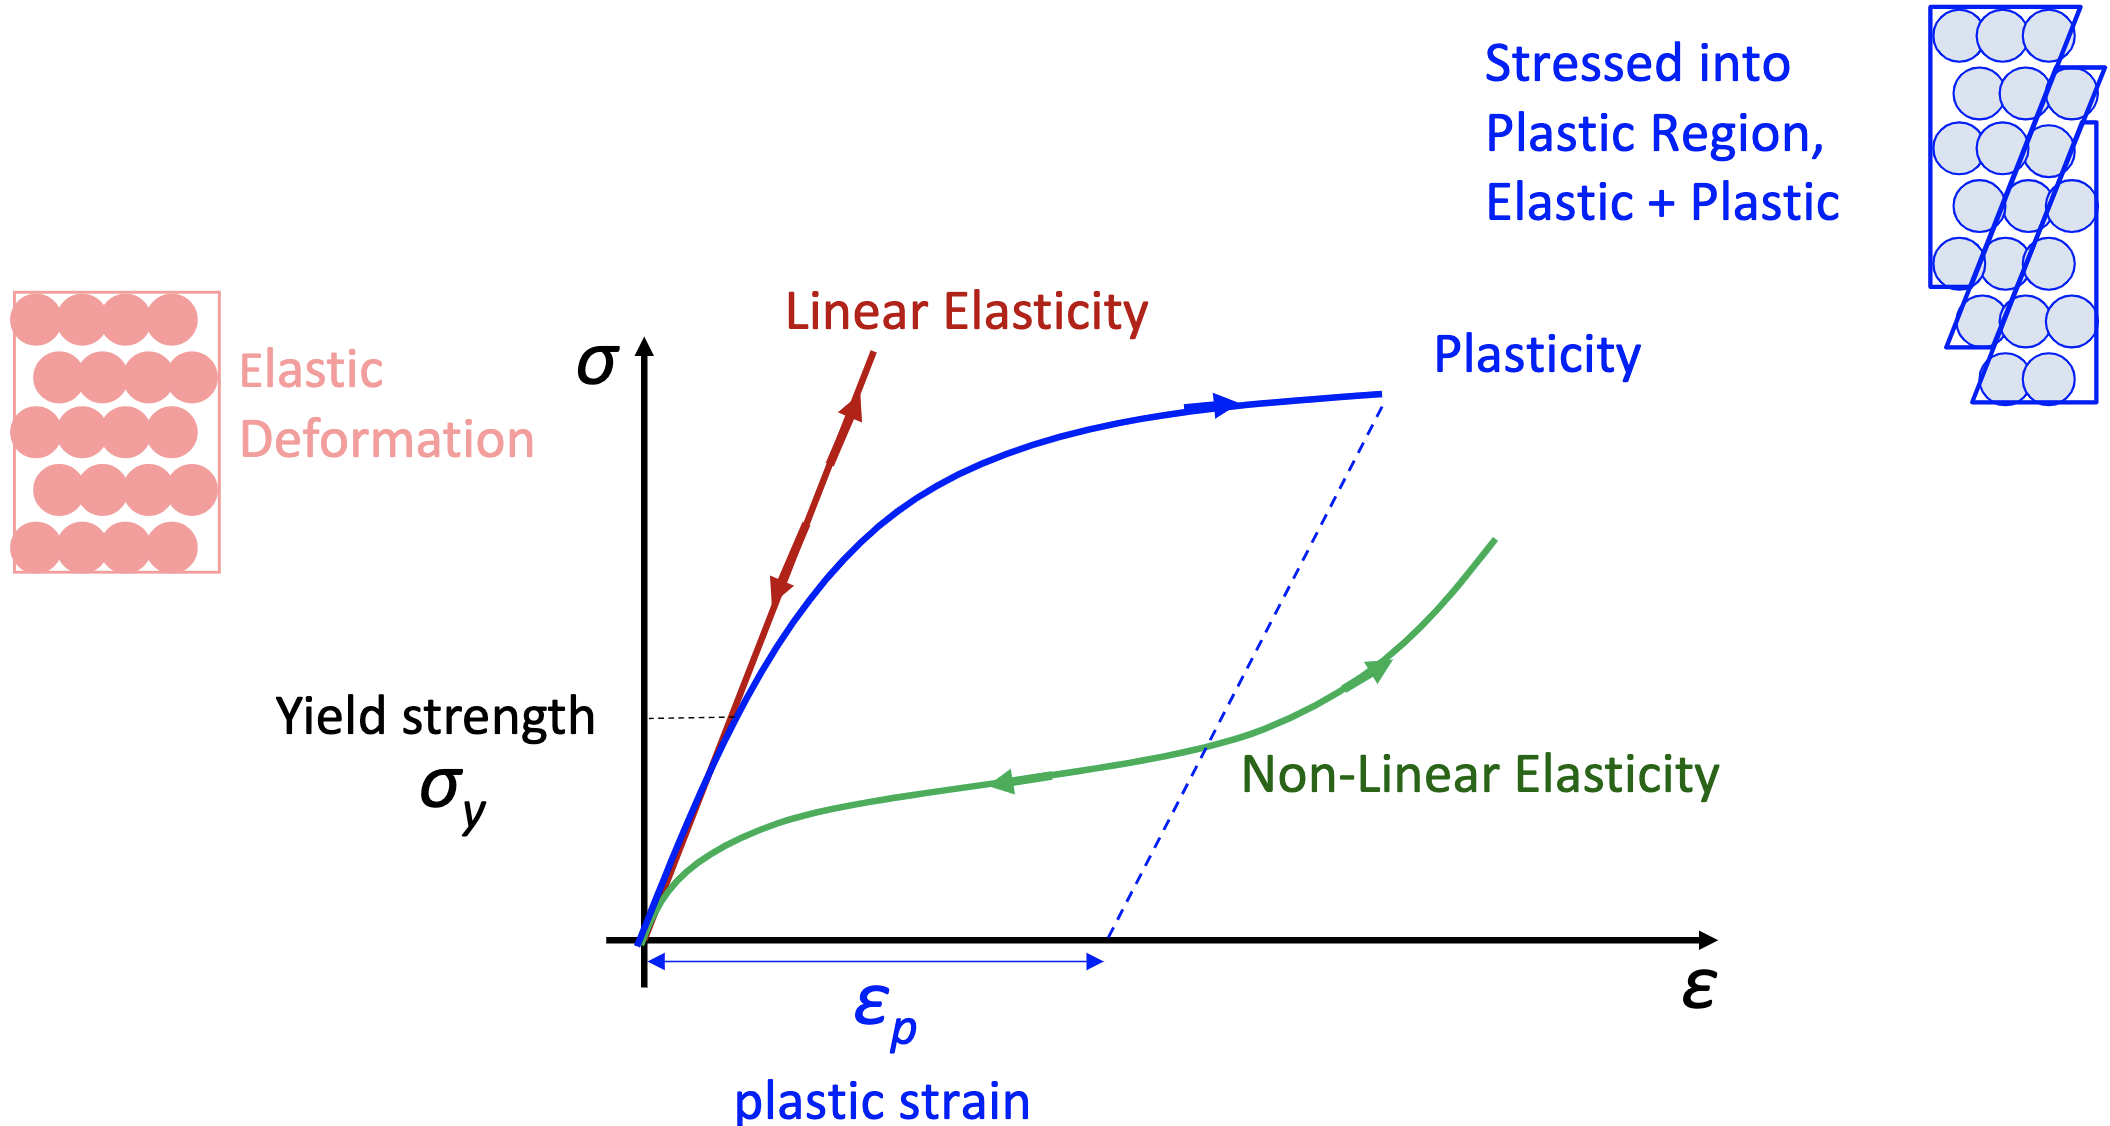
\includegraphics[width=0.6\linewidth]{./figures/f7_1.png}
  \label{fig:f7_1}
\end{figure}

\subsection{Stress-strain curves}
To get an understanding of how materials behave under increasing loads the following will provide a short explanation of a so-called \textit{stress-strain curve} (in this case for steel). The stress-strain curve can be seen on \textbf{\autoref{fig:f7_2}}.

\begin{figure} [ht]
  \centering
  \caption{Stress-strain curve for steel}
  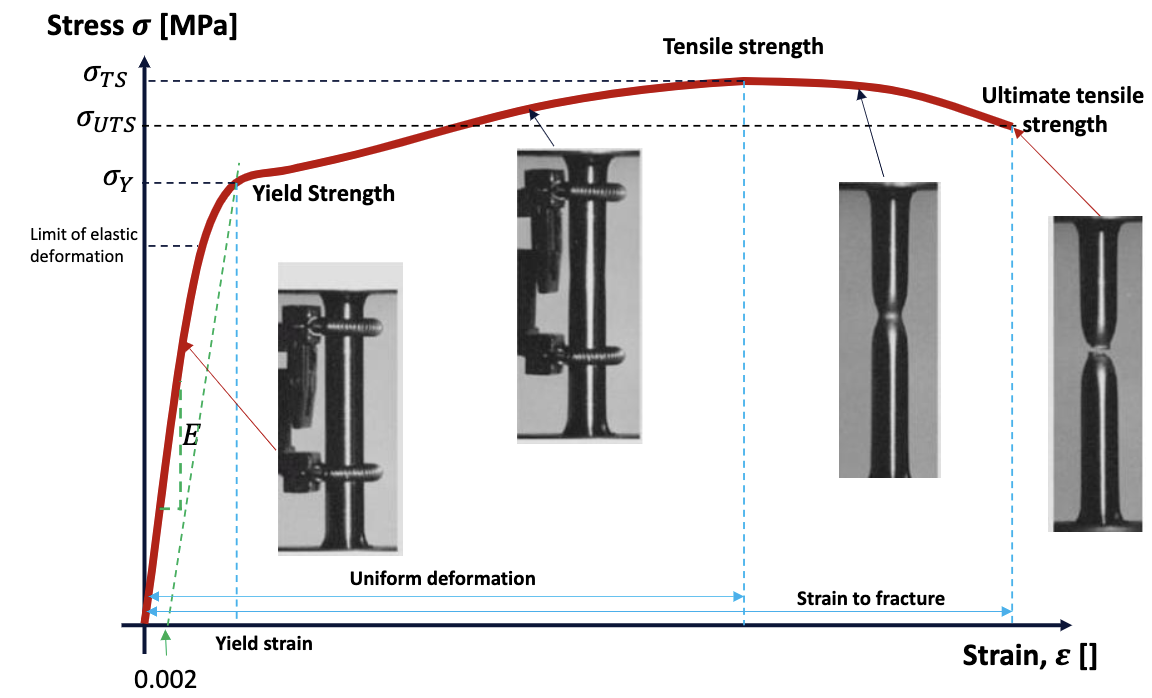
\includegraphics[width=0.7\linewidth]{./figures/f7_2.png}
  \label{fig:f7_2}
\end{figure}

\begin{itemize}
  \item When the load is applied (and has a relatively low size) the steel undergoes plastic deformation. During this phase of the process the stress increases linearly with the strain with a slope equal to Young's modulus for the material. 
  \item When the stress-strain curve stops being linear we have reached the limit of elastic deformation. Hereafter the material will (in theory) start to deform permanently.
  \item After increasing the load even more we reach the yield strength which is defined as having \textit{noticeable} deformation even after the stress is removed (this is often defined to \num{0,2} \%). The corresponding stress and strain (without removed load) at this point are known as the \textit{yield strength} and the \textit{yield strain}. 
  \item Hereafter the material will start to heavily deform and the stress-strain curve becomes ``flatter'', meaning less stress is required to produce additional strain.
  \item When the stress-strain curve reaches a maximum the tensile strength has been reached. For metals this point occurs right at the onset of visible ``necking'' (the metal becomes thinner and thinner around the point it is going to break). 
  \item After passing the tensile strength the stress will actually become lower again before reaching the ultimate tensile strength right at the point of fracture. 
\end{itemize}

\subsection{Elastic strain recovery and ductility}
As mentioned above, a material loaded beyond the elastic limit will start to deform permanently. After removing the load from the material the stress will return to zero along with the elastic strain. The plastic strain, however, will remain. This can actually be used to harden materials through the process of \textit{strain-hardening}. A graph of this is shown on \textbf{\autoref{fig:f7_3}}.

\begin{figure} [ht]
  \centering
  \caption{Elastic strain recovery}
  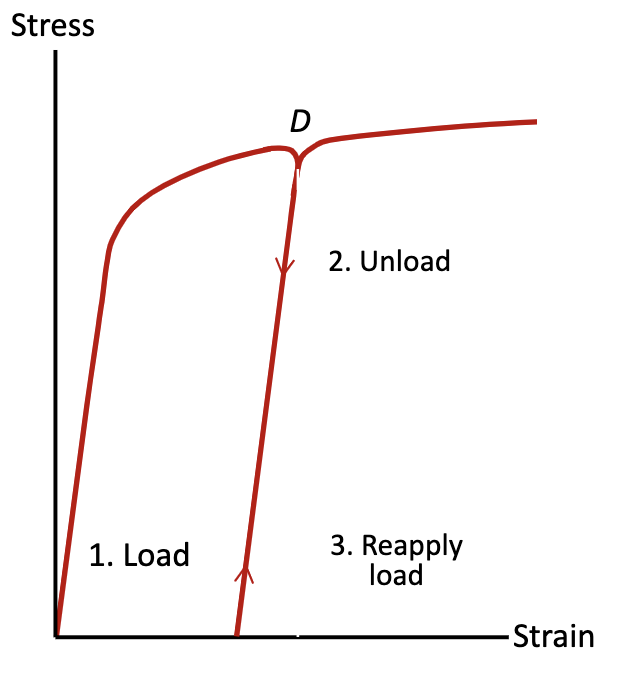
\includegraphics[width=0.5\linewidth]{./figures/f7_3.png}
  \label{fig:f7_3}
\end{figure}

The maximum amount of plastic deformation (amount of plastic deformation at failure) of a material is known as the materials \textit{ductility}. Ductility is normally measured in percent elongation or percent reduction in cross-sectional area. A material with high ductility will deform more before breaking then a material with lower ductility. 

\subsection{Resilience}
A materials \textit{resilience} is its ability to absorb energy during elastic deformation -- in other words it is the area underneath the stress-strain curve from 0 to the yield strain. This also corresponds to the amount of energy released when the load is removed (the potential energy in all the small springs that make up intermolecular bonds). Resilience is given by the \textit{modulus of resilience}, $U_r$. If we assume a linear stress-strain curve up till the yield strength we get a strain curve given by
\[ 
\sigma = E\epsilon
\]
which simplifies to
\[ 
U_r = \frac{1}{2}\sigma_y \epsilon_y = \frac{\sigma_y^2}{2E}
.\]

\subsection{Toughness}
A materials \textit{toughness} is a measurement of its ability to absorb energy before failure -- in other words it is equal to the area under the stress-strain curve. Materials with a smaller toughnesses will either break with little strain or strain with little stress -- think ceramics (break under small strain) or polymers (strain under small stress). Materials with high toughness will however both require a lot of stress before straining and strain for a long distance before breaking -- think many metals.

It should be noted that it is a common misconception that the toughness of a material inherently is related to whether a material is brittle or not. A small toughness does not necessarily mean a material is more brittle (e.g. will many polymers often have low toughness but still not be brittle, as they have the ability to plastically deform).


\subsection{Hardness}
A materials \textit{hardness} is a measure of the materials ability to withstand plastic deformation on its surface -- this can be either via indentation or scratches. A large hardness means a material is more resistant to compressive loads and oftentimes a harder material will have better wear properties.


\subsubsection{Hardness measurements}
Hardness is oftentimes measured on the qualitative \textit{Moh's scale}. This scale is determined by a materials ability to scratch another material -- in this way the Moh's scale is a comparative scale. The scale goes from 1 (talc) to 10 (diamond) and after making these two definitions one can place all other materials on the scale from 1-10 depending on which other materials a material can scratch.

However, different types of quantitative tests have also been designed to combat the qualitativeness og the Moh's scale. These generally all work by pressing an indenter (with specified material and size) into a sample with a given load before measuring the amount of plastic (permanent) deformation after removing the load. An example of such a quantitative test is the so-called \textit{Brinell Hardness scale}, which gives a hardness reading $\mathrm{HB}$. The Brinell test works by pressing a $D = \qty{10}{mm}$ sphere of steel or tungsten carbide into the material with a load of $P \, [\unit{kg}]$, which will leave a circular mark with diameter $d$. Thereafter the hardness ($\mathrm{HB}$-value) can be found as
\[ 
\mathrm{HB} = \frac{2P}{\pi D \left( D - \sqrt{D^2 - d^2} \right)}
.\]
In general there is a relationship between a materials Brinell hardness ($\mathrm{HB}$) and its tensile strength ($TS$) given by
\[ 
  TS \, \unit{MPa} \approx \num{3,45} \cdot \mathrm{HB}
.\]

Using the \textit{Vicker's microhardness scale} or the \textit{Knoop microhardness scale} instead of the Brinell scale, one would get an $\mathrm{HV}$ or $\mathrm{HK}$ value respetively. These can be found with
\begin{align*}
  \mathrm{HV} &= \num{1.854} \frac{P}{d_1^2} \\
  \mathrm{HK} &= \num{14,2} \frac{P}{l^2}
.\end{align*}

\textit{Note:} For the Vicker's scale $d_1$ is the sidelength of the pyramid-shaped indenter and for Knoop's scale $l$ is the length of the longest diagonal in the skew-pyramid-shaped indenter.


\subsection{Variability in materials properties}
Material properties always have some inherent randomness -- you cannot expect two different lumps of the same material to have exactly the same grain structure and so on. This means that a lump of a given material can have rather different properties. For this reason one needs to use a bit of statistical modelling when trying to measure a property. One can find the typical value, $\overline{x}$, by averaging all of ones $n$ different measurements, $x_i$, as
\[ 
  \overline{x} = \frac{\sum_{i = 1}^{n} x_i}{n}
.\]
This can then be used to find the \textit{sample standard deviation}, $s$, as
\[ 
s = \sqrt{\frac{\sum (x_i - \overline{x})}{n-1}}
.\]

\subsubsection{Safety factor}
Because of the inherent variability of a materials properties one must compensate for possibly getting a bad material to protect against unticipated failure. This is simply done by using the working stress $\sigma_w$ instead of the yield strength $\sigma_y$. To find this $\sigma_w$ one must also define a factor of safety $N$. Then the formula is
\[ 
\sigma_w = \frac{\sigma_y}{N}
.\]
The value of $N$ is typically between \num{1,2} and 4 depending on the application.
